\subsection{Chess Environment}
\label{subsec:chess}
\begin{wrapfigure}{r}{0.5\columnwidth}
\vspace{-3ex}
    \centering%
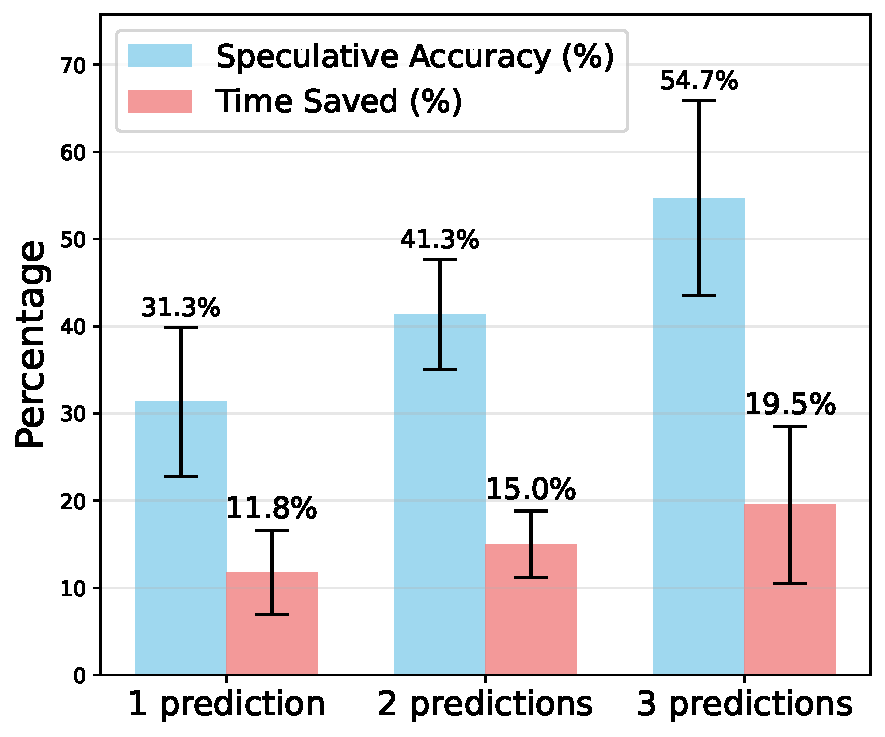
\includegraphics[width=0.9\linewidth]{figures/chess/combined_bar_plots.pdf}
  \caption{Percentage of time saved and percentage of correct predictions across $5$ runs at $30$ steps.}
  \vspace{-2em}
  \label{fig:chess_bar_plots}
\end{wrapfigure}
We demonstrate the effectiveness of our  framework in the context of competitive multi-agent gameplay, focusing on chess as a canonical turn-based example. In standard play, analysis is strictly sequential: each player begins analysis only \textit{after} the opponent has completed their turn. This serialization introduces substantial idle time. Particularly when both players rely on computationally intensive reasoning models, a single game can stretch to hours of wall-clock time. Our framework relaxes this constraint through speculative parallel analysis, allowing players to anticipate and prepare for likely opponent moves in advance. We show that this results in significant reductions in overall game duration.


% This strict serialization makes chess an ideal testbed for demonstrating how speculation can parallelize inherently sequential interactions.


\subsubsection{Implementation}

We implement our framework on top of TextArena \citep{guertler2025textarena}, which provides a standardized game-play interface for LLM-driven agents.

\textbf{Speculative Pipeline}. At turn $t$, the game state $s_t$ corresponds to the current board position. The in-turn player issues an API call $h_t$ with parameter $q_t$ constructed from $s_t$ together with a reasoning-eliciting prompt. At this point, player $P$ is to move, and player $Q$ awaits. Our framework  proceeds as follows:
\begin{itemize}[leftmargin=*]
    \item Current in-turn player $P$: the player receives $s_t$, makes an API call $h_t$ to the agent with parameter $q_t = (s_t, {prompt})$. This API call returns the next move $a_t = h(q_t)$, typically with high latency due to deep and extensive reasoning.
    \item Other out-of-turn player $Q$:
    \begin{enumerate}
        \item \textbf{Prediction phase}. The Speculator also receives the board state $s_t$ and issues an API call $\hat{h}_t$, using a prompt optimized for speed rather than depth. It returns the top-$k$ move predictions $\hat{a}_t^{(1)}, \hat{a}_t^{(2)}, \dots, \hat{a}_t^{(k)}$, ordered by confidence.
        \item \textbf{Parallel Computation}. For each predicted move $\hat{a}_t^{(i)}$, the out-of-turn player $Q$ immediately launches a parallel process analyzing a next move $\hat{a}_{t+1}^{(i)} = h_{t+1}(\hat{s}_{t+1}, {prompt})$ for $i \in \{1, \ldots, k\}$, where $ \hat{s}_{t+1}^{(i)} = f(s_t,\hat{a}_t^{(i)})$ denotes the next state resulting from applying predicted action $\hat{a}_t^{(i)}$ to $s_t$. 
        \item \textbf{Validation}. When the current in-turn player $P$ finishes reasoning and returns its move $a_t$, we immediately check whether it matches any of the predicted moves $\hat{a}_t^{(1)}, \hat{a}_t^{(2)}, \dots, \hat{a}_t^{(k)}$. 
        \item \textbf{Commit or Restart}.If a match exists, we commit to the corresponding speculative branch, advancing directly to $s_{t+1} = f(s_t, a_t)$. The game thus skips ahead, terminating other threads. If no match exists, we discard all speculative branches and continue with $Q$’s regular move computation $a_{t+1} = h_{t+1}(f(s_{t},a_t),{prompt})$. 
    \end{enumerate}
\end{itemize}

This pipeline is \textit{lossless}: the final trajectory remains identical to non-speculative play, but time is saved through parallelized reasoning.

\textbf{Agent Configuration} We find that using the same model for both Speculator and Actor, but with different prompts, maximizes prediction accuracy while keeping speculation fast. Accordingly, in our experiments, the Actor is instantiated as GPT-5 with high reasoning effort, with each move is produced via an API call. The Speculator also employs GPT-5, but configured with low reasoning effort and a specialized system prompt designed for rapid move prediction rather than exhaustive analysis.


\subsubsection{Results}
We evaluate our framework in terms of both time saved and prediction accuracy.

We track two metrics: (i) prediction accuracy, defined as the fraction of rounds in which any speculative prediction matches the actual move, and (ii) time saved, computed as $(T_{seq}-T_{s})/T_{seq}$, where $T_{s}$ and $T_{seq}$ denote speculative and sequential execution times, respectively.


\textbf{Time Saved and Accuracy increases with more predictions.}
Figure~\ref{fig:chess_bar_plots} reports results over 30 steps. Our framework consistently reduces execution time compared to sequential play, with larger savings as the number of speculative predictions increases. Across 5 runs, using 3 predictions yields an average time saving of $19.5\%$ with an average prediction accuracy of $54.7\%$.

\textbf{Randomness of agent call in game-play}
Variance in Figure~\ref{fig:chess_bar_plots} reflects realistic game-play dynamics from actual game runs with live API calls. Even with correct predictions, time savings vary: when the resulting position admits an obvious response, little acceleration occurs, as computation would be fast regardless. Significant gains arise only when predictions lead to positions requiring deep analysis. Thus, the effectiveness of speculation depends jointly on prediction accuracy and the complexity of the resulting positions.